
% This LaTeX was auto-generated from an M-file by MATLAB.
% To make changes, update the M-file and republish this document.

\documentclass{article}
\usepackage{graphicx}
\usepackage{color}

\sloppy
\definecolor{lightgray}{gray}{0.5}
\setlength{\parindent}{0pt}

\begin{document}

    
    
\subsection*{Contents}

\begin{itemize}
\setlength{\itemsep}{-1ex}
   \item read the images
   \item embed background behind person
   \item embed person in background image
\end{itemize}
\begin{verbatim}
clc;
close all;
\end{verbatim}


\subsection*{read the images}

\begin{verbatim}
i = imread('me2.jpg');
figure;
imshow(i);

b = imread('/home/vaishali/Desktop/colosseum.jpg');
figure;
imshow(b);
\end{verbatim}

        \color{lightgray} \begin{verbatim}Warning: Image is too big to fit on screen; displaying at 17% 
\end{verbatim} \color{black}
    
\includegraphics [width=4in]{chromaKey_01.eps}

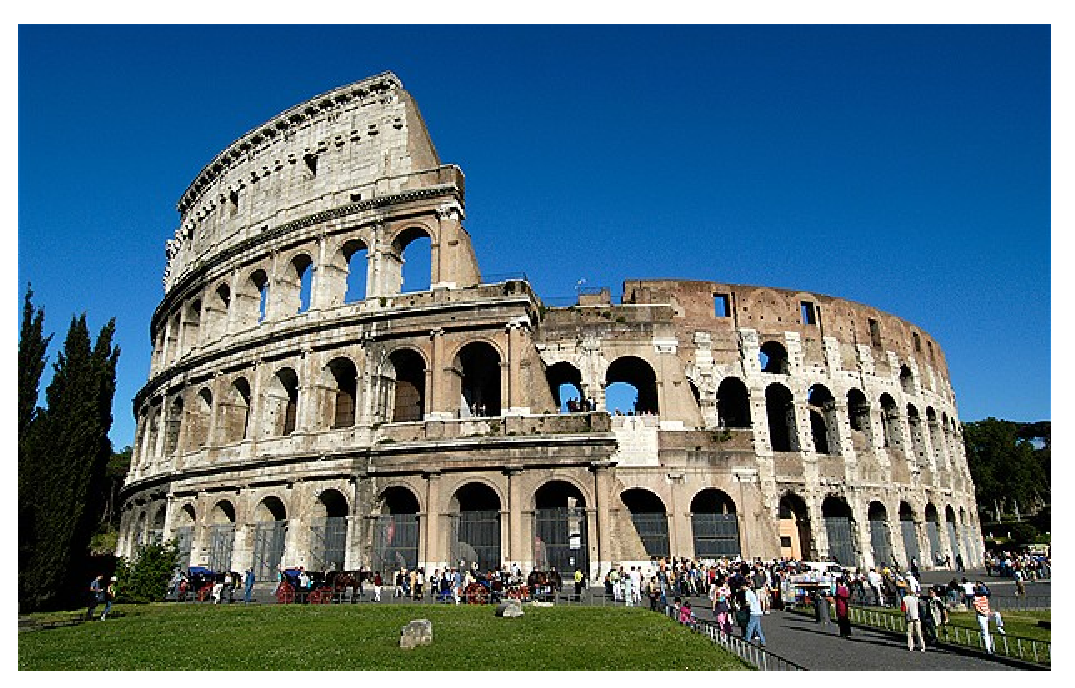
\includegraphics [width=4in]{chromaKey_02.eps}


\subsection*{embed background behind person}

\begin{verbatim}
b = imresize(b, [size(i,1) size(i,2)]);

%insert background image in person image
for q = 1: size(i,2)
    for p = 1: size(i,1)
        if(i(p,q,1) > 100 && i(p,q,2) > 100 && i(p,q,3) > 100 && i(p,q,1) < 200 && i(p,q,2) < 200 && i(p,q,3) < 200)
            i(p,q,:) = b(p,q,:);
        end
    end
end

figure;
imshow(i);
\end{verbatim}

        \color{lightgray} \begin{verbatim}Warning: Image is too big to fit on screen; displaying at 17% 
\end{verbatim} \color{black}
    
\includegraphics [width=4in]{chromaKey_03.eps}


\subsection*{embed person in background image}

\begin{verbatim}
%read image
i = imread('me2.jpg');
b = imread('/home/vaishali/Desktop/colosseum.jpg');
i = imresize(i, 0.125);

% coordinates for translation of foreground image
x = size(b,1)-size(i,1);
y = size(b,2)-size(i,2);

%insert person image in background image
for p = 1:size(i,1)
    for q = 1:size(i,2)
        if(~(i(p,q,1) > 110 && i(p,q,2) > 110 && i(p,q,3) > 110 && i(p,q,1) < 200 && i(p,q,2) < 200 && i(p,q,3) < 200))
            b(p+x,q,:) = i(p,q,:);
        end

    end
end
figure;
imshow(b);
\end{verbatim}

\includegraphics [width=4in]{chromaKey_04.eps}



\end{document}
    
